\documentclass{beamer}
\usepackage{relsize}
\usepackage{color}

\usepackage{listings}
\usetheme{CambridgeUS}
%\usepackage{beamerthemesplit} % new 
\usepackage{enumitem}
\usepackage{amsmath}                    % See geometry.pdf to learn the layout options. 
\usepackage{amsthm}                   % See geometry.pdf to learn the layout options. There 
\usepackage{amssymb}                    % See geometry.pdf to learn the layout options. 
\usepackage[utf8]{inputenc} 
\usepackage{graphicx}
\usepackage[english,bulgarian]{babel}

\lstset{language=C++,
                basicstyle=\ttfamily,
                keywordstyle=\color{blue}\ttfamily,
                stringstyle=\color{red}\ttfamily,
                commentstyle=\color{green}\ttfamily,
                morecomment=[l][\color{magenta}]{\#}
}

\newtheorem{mydef}{Дефиниция}[section]
\newtheorem{lem}{Лема}[section]
\newtheorem{thm}{Твърдение}[section]

\DeclareMathOperator{\restrict}{\upharpoonright}

\setitemize{label=\usebeamerfont*{itemize item}%
  \usebeamercolor[fg]{itemize item}
  \usebeamertemplate{itemize item}}

\setbeamercovered{transparent}



\begin{document}
\title[Увод в програмирането]{Указатели. Маисиви, указатели, параметри на функции} 
\author{Калин Георгиев} 
\frame{\titlepage} 



\begin{frame}
\centerline{Указатели!}
\end{frame}



\begin{frame}[fragile]
\frametitle{Дефиниране}
\begin{flushleft}
\relscale{0.7}
\begin{lstlisting}
long a=1,b=2;
long *pi = &a;
\end{lstlisting}
\end{flushleft}

\begin{center}
  

\begin{tabular}{c | c | c | c | c}
... & 100 & 104 & 108 & ...\\\hline
... & a   & b   & pi  & ... \\\hline
... & 1   & 2   & 100 & ... \\
  
\end{tabular}
\end{center}
\end{frame}


\begin{frame}[fragile]
\frametitle{Операции: ``през'' указател, \underline{С} указател}


\begin{columns}[t]
  \begin{column}{0.5\textwidth}

\begin{center}
  
\begin{tabular}{c | c | c | c | c}
... & 100 & 104 & 108 & ...\\\hline
... & a   & b   & pi  & ... \\\hline
... & 1   & 2   & 100 & ... \\
  
\end{tabular}
\end{center}


\begin{flushleft}
\relscale{0.7}
\begin{lstlisting}
*pi = 10;
\end{lstlisting}
\end{flushleft}

\pause

\begin{center}
  
\begin{tabular}{c | c | c | c | c}
... & 100 & 104 & 108 & ...\\\hline
... & a   & b   & pi  & ... \\\hline
... & \alert{10}   & 2   & 100 & ... \\
  
\end{tabular}
\end{center}


  \end{column}
  \begin{column}{0.5\textwidth}

\pause
\begin{flushleft}
\relscale{0.7}
\begin{lstlisting}
pi = 104; //won't compile
\end{lstlisting}
\end{flushleft}

\begin{center}
  
\pause

\begin{tabular}{c | c | c | c | c}
... & 100 & 104 & 108 & ...\\\hline
... & a   & b   & pi  & ... \\\hline
... & 10  & 2   & \alert{104} & ... \\
  
\end{tabular}
\end{center}

\pause

\begin{flushleft}
\relscale{0.7}
\begin{lstlisting}
*pi = 104; 
\end{lstlisting}
\end{flushleft}

\begin{center}
  
\pause

\begin{tabular}{c | c | c | c | c}
... & 100 & 104 & 108 & ...\\\hline
... & a   & b   & pi  & ... \\\hline
... & 10  & \alert{104}   & 104 & ... \\
  
\end{tabular}
\end{center}
  \end{column}
\end{columns}



\end{frame}


\begin{frame}[fragile]
\frametitle{Пример с функции}
\begin{columns}[t]
  \begin{column}{0.4\textwidth}
\begin{flushleft}
\relscale{0.7}
\begin{lstlisting}
void f (long x)
{
  x = x + 10; //(2')
  cout << x;
}

void g (long *px)
{
  *px = *px + 10; //(5)
  cout << *px;
}

long main ()
{
  long x = 0; //(1)
  f(x);      //(2)
  cout << x; //(3)
  g (&x);    //(4)
  cout << x; //(6)
}
\end{lstlisting}
\end{flushleft}

  \end{column}
  \begin{column}{0.3\textwidth}

  (1)main:

  \begin{tabular}{c|c}
  x & 0 
  \end{tabular}

\pause

  \vspace{10px}
  (2,2')main:

  \begin{tabular}{c|c}
  x & 0 
  \end{tabular}

  f:

  \begin{tabular}{c|c}
  x & 0 \\\pause
  x & \alert {10}
  \end{tabular}

\pause

  \vspace{10px}
  (3)main:

  \begin{tabular}{c|c}
  x & 0 
  \end{tabular}

\pause

  \vspace{10px}
  (4)main:

  \begin{tabular}{c|c}
  x & 0 
  \end{tabular}

  g:

  \begin{tabular}{c|c}
  px & 100 
  \end{tabular}



  \end{column}
  \begin{column}{0.3\textwidth}

\pause

  (5)main:

  \begin{tabular}{c|c}
  x & \alert{10} 
  \end{tabular}

  g:

  \begin{tabular}{c|c}
  px & 100 
  \end{tabular}

\vspace{10px}
\pause

  (6)main:

  \begin{tabular}{c|c}
  x & 10
  \end{tabular}


  \end{column}


\end{columns}




\end{frame}

\begin{frame}[fragile]
\frametitle{Параметър по стойност vs. по указател}

\begin{flushleft}
\relscale{0.7}
\begin{lstlisting}
long division (long x, long y, long *remainder)
{
  *remainder = x - (x/y)*y;
  return x/y;
}

long main ()
{
  long r = 0;
  cout << "[14/4]=" 
       << division (14,4,&r)
       << "|14/4|="
       << r
       << endl;
}
\end{lstlisting}
\end{flushleft}

\end{frame}


\begin{frame}[fragile]
\frametitle{Какво е нередно в този пример?}

\begin{flushleft}
\relscale{0.7}
\begin{lstlisting}
long division (long x, long y, long *remainder)
....
\end{lstlisting}
\end{flushleft}


\begin{center}
\relscale{1.2}
\begin{lstlisting}
cout << division (2,2,0);
\end{lstlisting}
\end{center}


\end{frame}



\begin{frame}
\centerline{Масиви и указатели}
\end{frame}


\begin{frame}[fragile]
\frametitle{Какво е a? Какво е arr?}

\begin{flushleft}
\relscale{0.8}
\begin{lstlisting}
long a = 5; b = 10; long arr[3] = {1,2,3}; arr2[3] = {4,5,6};
\end{lstlisting}
\end{flushleft}

\pause

\begin{itemize}
  \item а  и  b: заместител на адреса / ``наименование'' на буфера
\end{itemize}

\begin{flushleft}
\relscale{0.8}
\begin{lstlisting}
a = 2; a = a + 3; b = a + b; if (a > b) {...}
\end{lstlisting}
\end{flushleft}

\pause

\begin{itemize}
  \item Операциите с масиви са операции с елементите им
  \item Отеделните елементи имат свойства на обикновени променливи от съответния тип
\end{itemize}

\begin{flushleft}
\relscale{0.8}
\begin{lstlisting}
arr[0] = 2; arr[0] = arr[1] + 3; ...
\end{lstlisting}
\end{flushleft}

\pause

\begin{itemize}
  \item Какво са arr и arr2 сами по себе си?
\end{itemize}


\begin{flushleft}
\relscale{0.8}
\begin{lstlisting}
arr = ???; arr2 = arr???; if (arr > arr2) ???
\end{lstlisting}
\end{flushleft}

\end{frame}


\begin{frame}[fragile]
\frametitle{Указател към първия елемент}


\begin{flushleft}
\relscale{0.8}
\begin{lstlisting}
long arr[3] = {1,2,3};
\end{lstlisting}
\end{flushleft}

\pause

\begin{tabular} {c | c | c | c | c | c }

arr &... &*arr \\\hline
80  &... & 100 & 104 & 108 &... \\\hline
100 &... & 1   & 2   & 3   &... \\\hline
  
\end{tabular}

\end{frame}




\begin{frame}[fragile]
\frametitle{Операции}


\begin{tabular} {c | c | c | c | c | c }

arr &... &*arr \\\hline
80  &... & 100 & 104 & 108 &... \\\hline
100 &... & 1   & 2   & 3   &... \\\hline
  
\end{tabular}


\begin{itemize}
  \item Отново ``писане и четене през'' указател
\begin{flushleft}
\relscale{0.8}
\begin{lstlisting}
*arr = 10;
cout << *arr;
\end{lstlisting}
\end{flushleft}

\end{itemize}

\pause
\begin{tabular} {c | c | c | c | c | c }

arr &... &*arr \\\hline
80  &... & 100 & 104 & 108 &... \\\hline
100 &... & \alert{10}   & 2   & 3   &... \\\hline
  
\end{tabular}

\end{frame}

\begin{frame}[fragile]
\frametitle{Адресна аритметика}


\begin{tabular} {c | c | c | c | c | c }

arr &... &*arr \\\hline
80  &... & 100 & 104 & 108 &... \\\hline
100 &... & 10   & 2   & 3   &... \\\hline
  
\end{tabular}


\begin{itemize}
  \item Аритметични операции с указател:   

\texttt{<указател>+<ест. число>=<указател>}
\begin{flushleft}
\relscale{0.8}
\begin{lstlisting}
*(arr+2) = 10;
\end{lstlisting}
\end{flushleft}

\end{itemize}

\pause
\begin{tabular} {c | c | c | c | c | c }

arr &... &*arr \\\hline
80  &... & 100 & 104 & 108 &... \\\hline
100 &... & 10   & 2   & \alert{10}   &... \\\hline
  
\end{tabular}

\end{frame}



\begin{frame}[fragile]
\frametitle{Още за адресната аритметика}


\begin{tabular} {c | c | c | c | c | c }

arr &... &*arr \\\hline
80  &... & 100 & 104 & 108 &... \\\hline
100 &... & 10   & 2   & 10   &... \\\hline
  
\end{tabular}

\vspace{15px}

\begin{itemize}
\item \texttt{arr+i == \&arr[i]}
\pause
\item \texttt{*(arr+i) <==> arr[i]}
\pause
\item \texttt{(long)(arr+1)==104 // != 101}
\end{itemize}

\pause

\begin{flushleft}
\relscale{0.8}
\begin{lstlisting}
char charArr[6] = "Hello";
\end{lstlisting}
\end{flushleft}

\begin{itemize}
  \item \texttt{(long)(charArr+1) - (long)(charArr+2) == 1 == sizeof(char)}
  \item \texttt{(long)(arr+1) - (long)(arr+2) == 4 == sizeof(long)}
  \item Слеводателно \texttt{arr[i] <==> *(arr+i)}, независимо от размера на елементите
\end{itemize}


\end{frame}




\begin{frame}[fragile]
\frametitle{Масиви и функции}

\begin{flushleft}
\relscale{0.8}
\begin{lstlisting}
long sum (long arr[])
{
  
  long sum = 0;
  for (int i = 0; i < 3; i++)
  {
    sum += arr[i];
  }
  return sum;
}

int main ()
{
  int a[3] = {1,2,3};
  int b[4] = {1,2,3,4};

  cout << sum(a) << " " << sum (b) << endl;
}

\end{lstlisting}
\end{flushleft}

\end{frame}


\begin{frame}[fragile]
\frametitle{Не можем да определим размера на масиви динамично}

\begin{flushleft}
\relscale{0.8}
\begin{lstlisting}
long sum (long arr[], int n)
{
  
  long sum = 0;
  for (int i = 0; i < n; i++)
  {
    sum += arr[i];
  }
  return sum;
}

int main ()
{
  int a[3] = {1,2,3};
  int b[4] = {1,2,3,4};

  cout << sum(a,3) << " " << sum (b,4) << endl;
}

\end{lstlisting}
\end{flushleft}

\end{frame}


\begin{frame}[fragile]
\frametitle{"Подмасиви"}

\begin{tabular} {c|c|c|c|c|c|c|c|c|c|c }

    &  c   &    & c+2 \\\hline
... &1     & 2  & \alert{3}  & \alert{4} & \alert{5} &  \alert{6} & 7 & 8 & 9 &...  \\\hline
  
\end{tabular}

\begin{flushleft}
\relscale{0.8}
\begin{lstlisting}

int main ()
{
  int c[8] = {1,2,3,4,6,7,8,9};

  cout << sum(c,4);
  cout << sum(c+2,4);
}

\end{lstlisting}
\end{flushleft}

\end{frame}


\begin{frame}[fragile]
\frametitle{Внимание! Странични ефекти! }

\begin{flushleft}
\relscale{0.8}
\begin{lstlisting}
void test (long arr[], long x)
//void test (long *arr, long x)
{
  
  x++;       
  arr[0]++; // <==> *arr=*arr+1
  arr[1]++; // <==> *(arr+1)=*(arr+1)+1

}

int main ()
{
 
  long arr[2]={0,1};
  long x = 0;
  test (arr,x);
  cout << arr[0];
  cout << x;

}

\end{lstlisting}
\end{flushleft}

\end{frame}


\begin{frame}
\centerline{Пример: Двоично търсене}
\end{frame}

\begin{frame}[fragile]
\frametitle{Алгоритъм на двоичното търсене}

%\vspace*{-120pt}
%\hspace*{-30pt}
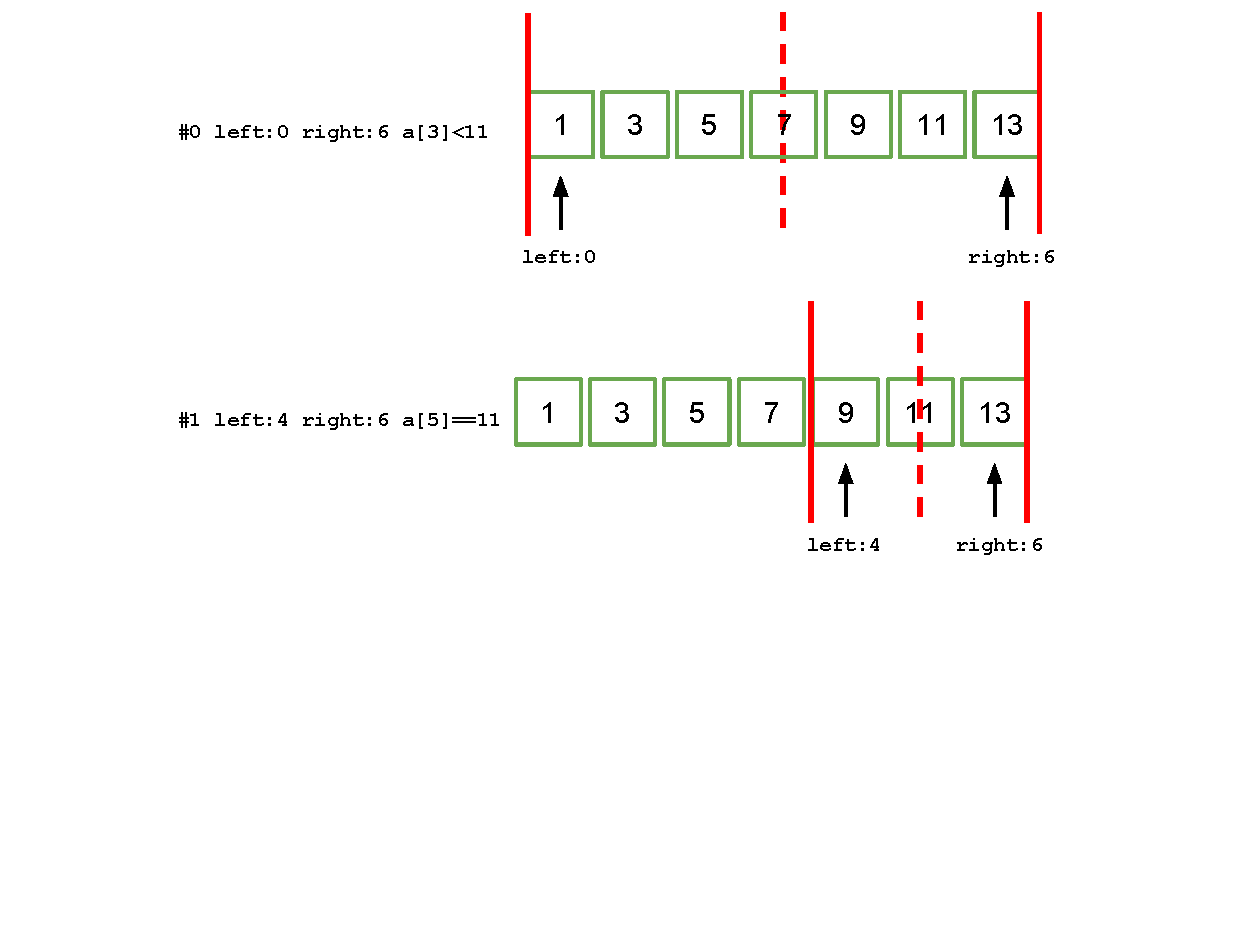
\includegraphics[width=14cm]{images/binsearch} 

\end{frame}



\begin{frame}[fragile]
\frametitle{Реализация с цикъл}



\begin{columns}[t]
  \begin{column}{0.5\textwidth}

\relscale{0.70}
\begin{lstlisting}
bool find (int x, int a[], int size)
{
  int left=0, right = size-1;

  while (left < right && 
         a[(left+right)/2] != x)
  {
    if (a[(left+right)/2] < x)
      left = (left+right)/2 + 1;
    else
      right = (left+right)/2;
  }

  return a[(left+right)/2] == x;
}
\end{lstlisting}


  \end{column}
  \begin{column}{0.5\textwidth}
\vspace*{-1pt}
\hspace*{-50pt}
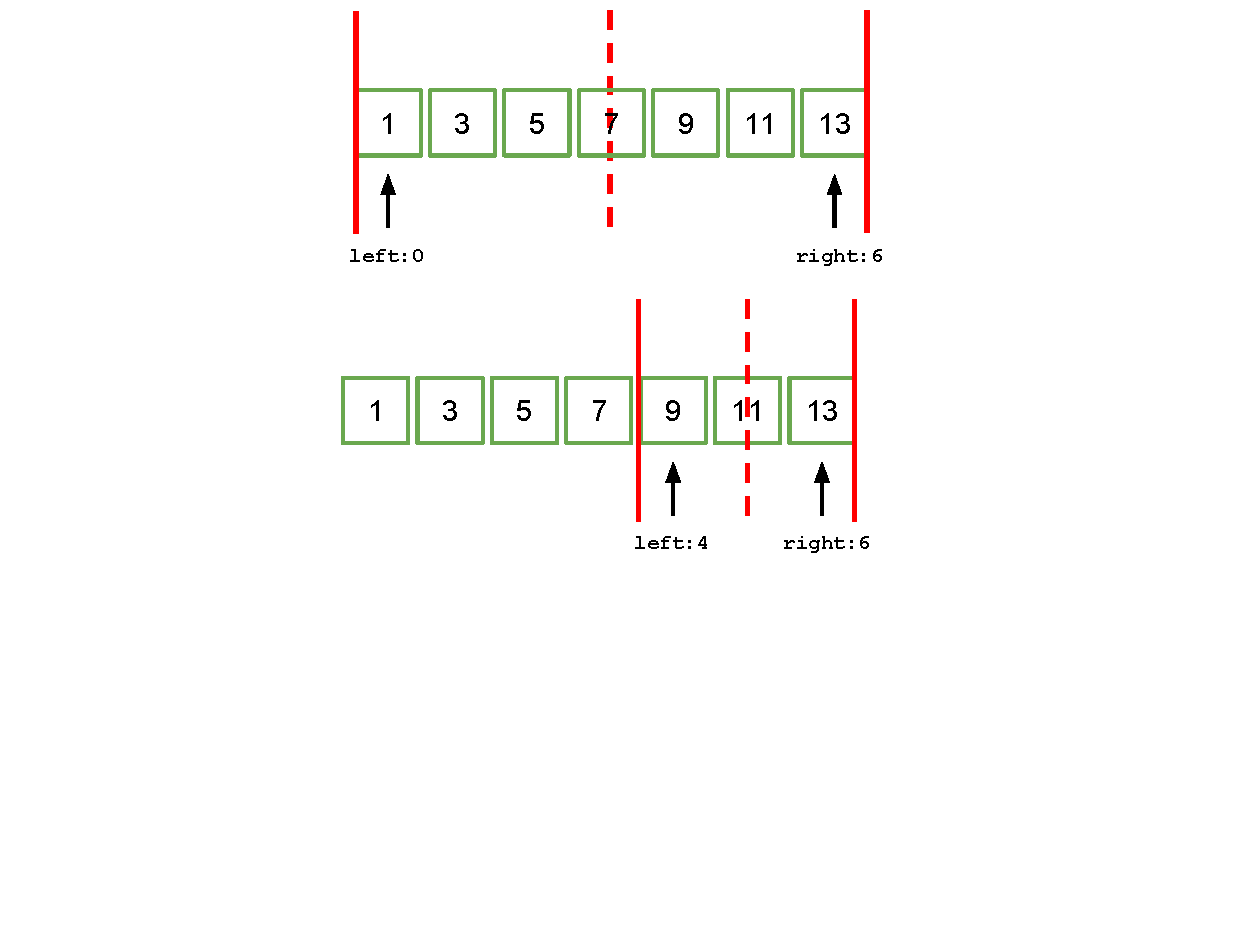
\includegraphics[width=10cm]{images/binsearch_smaller} 

  \end{column}
\end{columns}



\end{frame}






\begin{frame}[fragile]
\frametitle{Реализация с рекурсия}



\begin{columns}[t]
  \begin{column}{0.5\textwidth}

\relscale{0.70}
\begin{lstlisting}
bool findrec (int x, int a[], int size)
{
  if (size == 0)
  {
    return false;
  }
  if (size == 1)
  {
    return a[0] == x;
  }
  if (a[size/2] > x)
  {
    return findrec (x,a,size/2);
  }
  if (a[size/2] < x)
  {
    return findrec (x,a+(int)ceil(size/2.0),ceil(size/2.0)-1);
  }
  return true;
}
\end{lstlisting}


  \end{column}
  \begin{column}{0.5\textwidth}
\vspace*{-1pt}
\hspace*{-50pt}
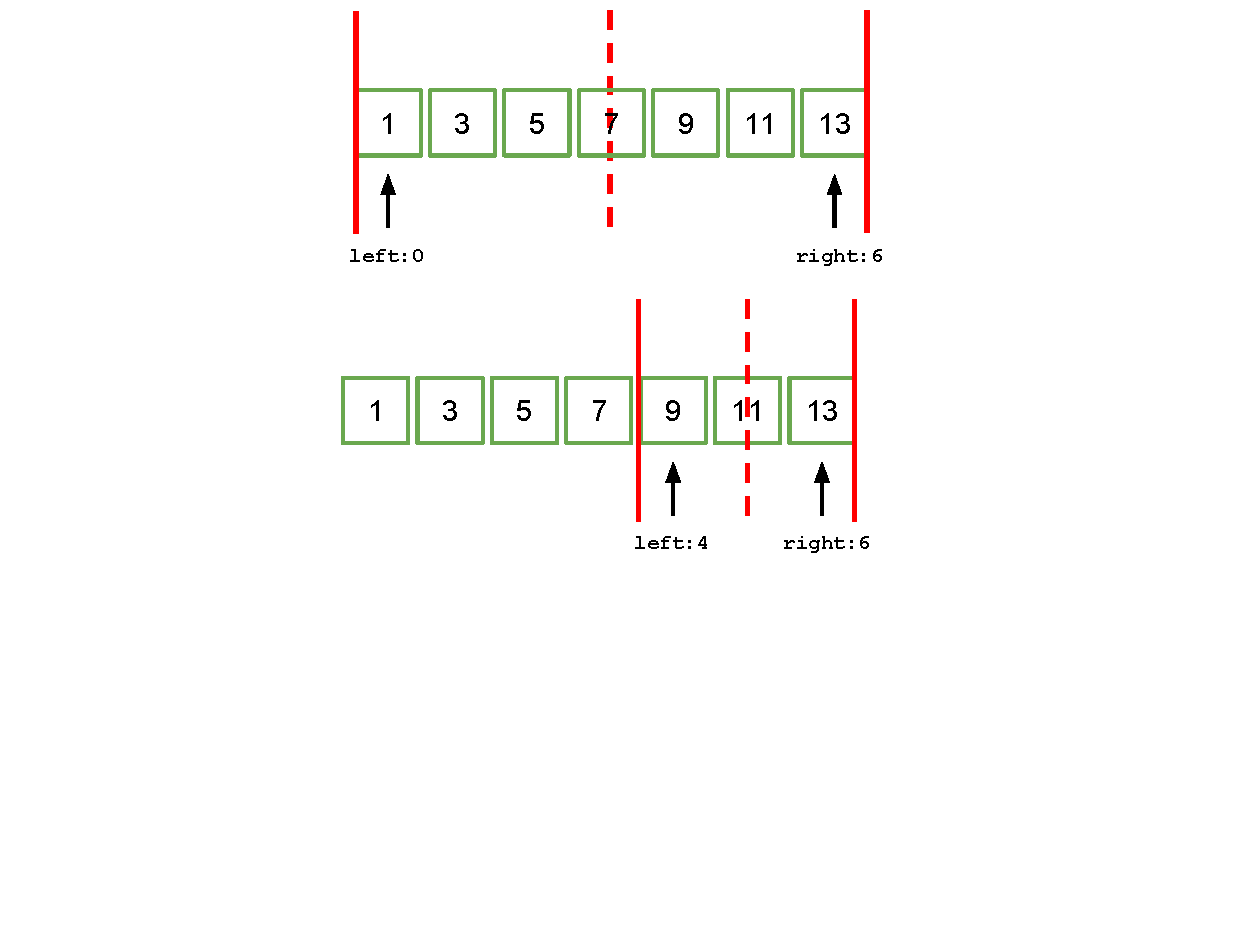
\includegraphics[width=10cm]{images/binsearch_smaller} 

  \end{column}
\end{columns}



\end{frame}


\begin{frame}[fragile]
\frametitle{А това защо работи?}



\begin{columns}[t]
  \begin{column}{0.5\textwidth}

\relscale{0.60}
\begin{lstlisting}
bool findreclogic (int x, int a[], int size)
{
  return 
  
  (size == 1 && 
   a[0] == x) ||


  (size > 1 && 
   a[size/2] > x && 
   findreclogic (x,a,size/2)) ||



  (size > 1 && 
   a[size/2] < x && 
   findreclogic (x,
                 a+(int)ceil(size/2.0),
                 ceil(size/2.0)-1))  ||
  

  (size > 1 && 
   a[size/2] == x);
}
\end{lstlisting}


  \end{column}
  \begin{column}{0.5\textwidth}
\vspace*{-1pt}
\hspace*{-50pt}
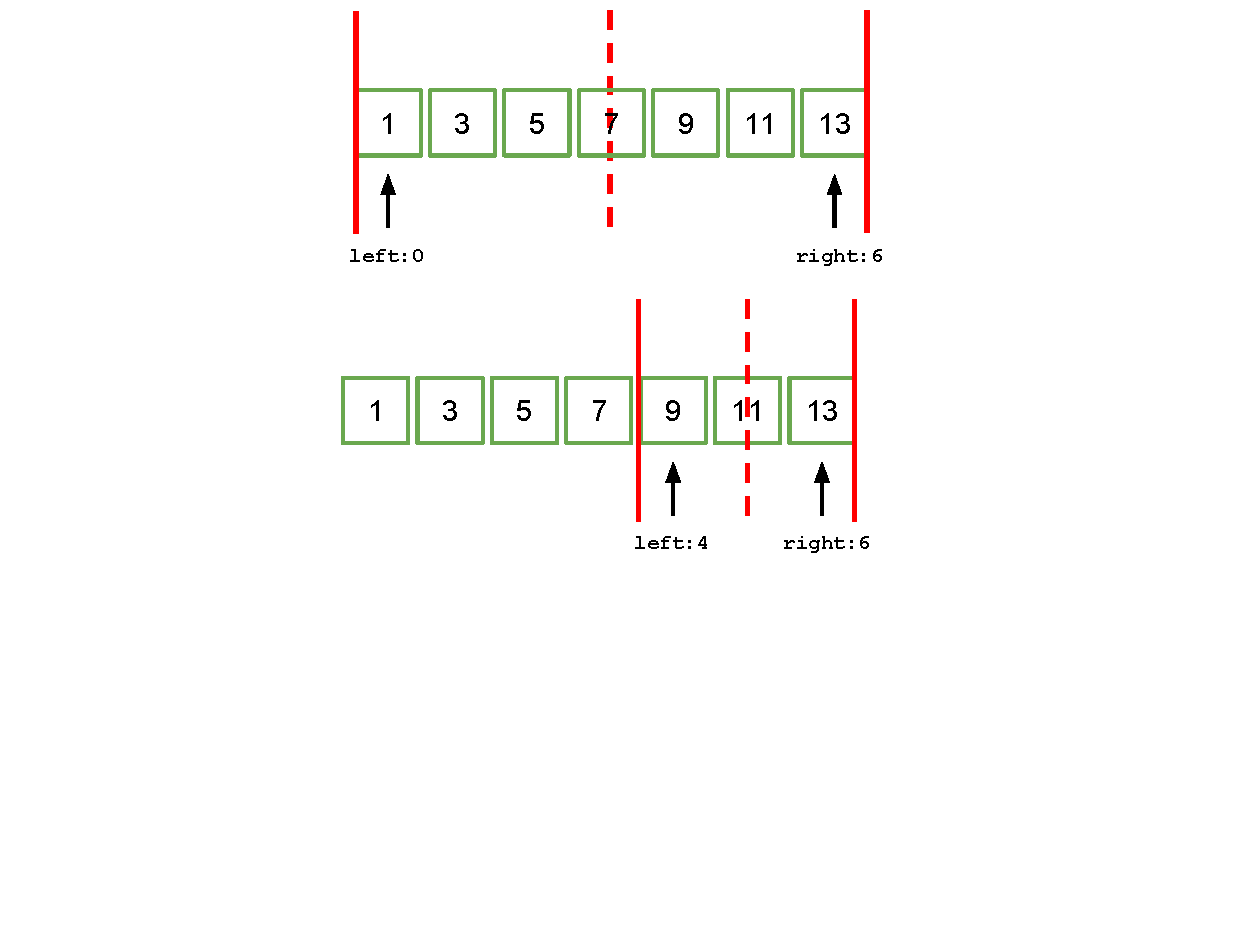
\includegraphics[width=10cm]{images/binsearch_smaller} 

  \end{column}
\end{columns}



\end{frame}



\begin{frame}
\centerline{Благодаря за вниманието!}
\end{frame}


\end{document}

